\documentclass[12pt]{article}
%\usepackage[utf8]{inputenc}
%\documentclass[UTF8]{ctexart}
%\usepackage[UTF8, heading = false, scheme = plain]{ctex}
\usepackage{geometry}
%geometry{a4paper,scale=0.9}
\geometry{a4paper,left=1cm,right=1cm,top=1cm,bottom=2cm}
\usepackage{amsfonts}
\usepackage{color}
\usepackage{url}
%\usepackage{biblatex}
\usepackage{amsmath}
\usepackage{amssymb}
\usepackage{latexsym}
\usepackage{cite}
%\addbibresource{ref.bib}
%\bibliography{ref.bib}
\usepackage{caption}
\usepackage{graphicx, subfig}
\usepackage{float}
%\usepackage[fontset=ubuntu]{ctex}
%\usepackage{fontspec}
\usepackage{xeCJK}
%\usepackage[colorlinks,
%anchorcolor=black,
%citecolor=black]{hyperref}
%\setmainfont{SimSun}
\usepackage[section]{placeins}
\usepackage{enumitem}
\usepackage{framed}
\usepackage[framemethod=TikZ]{mdframed}
\usepackage{indentfirst}
\usepackage{setspace}%使用间距宏包
\linespread{1.5}

\title{消息队列}
\author{leolinuxer}
%\date{June 2020}

\begin{document}
%\setlength{\parindent}{0pt}
\maketitle
\tableofcontents

\section{消息队列积压\cite{Message_Queue_Accident}}
\subsection{问题背景}
如何解决消息队列的延时以及过期失效问题?消息队列满了以后该怎么处理?有几百万消息持续积压几小时,说说怎么解决?


\subsection{问题原因}
其实本质针对的场景,都是说,可能你的消费端出了问题,不消费了,或者消费的极其极其慢。可能有以下原因:
\begin{itemize}
\setlength{\itemsep}{0pt}
\setlength{\parsep}{0pt}
\setlength{\parskip}{0pt}
    \item 可能你的消息队列集群的磁盘都快写满了,都没人消费;
    \item 或者是你积压的时间太长了,导致比如rabbitmq设置了消息过期时间后就没了;
    \item ……
\end{itemize}

所以这类问题其实线上挺常见的,一般不出,一出就是大case,一般常见于,举个例子,消费端每次消费之后要写mysql,结果mysql挂了,消费端hang那儿了,不动了。或者是消费端出了个什么叉子,导致消费速度极其慢。

\subsection{问题解法}
\subsubsection{大量消息在mq里积压了几个小时了还没解决}
几千万条数据在MQ里积压了七八个小时,从下午4点多,积压到了晚上很晚,10点多,11点多。这个是我们真实遇到过的一个场景,确实是线上故障了,这个时候要不然就是修复consumer的问题,让他恢复消费速度,然后傻傻的等待几个小时消费完毕。这个肯定不能在面试的时候说吧。

一个消费者一秒是1000条,一秒3个消费者是3000条,一分钟是18万条,1000多万条。所以如果你积压了几百万到上千万的数据,即使消费者恢复了,也需要大概1小时的时间才能恢复过来。

一般这个时候,只能操作临时紧急扩容了,具体操作步骤和思路如下:

(1)先修复consumer的问题,确保其恢复消费速度,然后将现有cnosumer都停掉;

(2)新建一个topic,partition是原来的10倍,临时建立好原先10倍或者20倍的queue数量;

(3)然后写一个临时的分发数据的consumer程序,这个程序部署上去消费积压的数据,消费之后不做耗时的处理,直接均匀轮询写入临时建立好的10倍数量的queue;

(4)接着临时征用10倍的机器来部署consumer,每一批consumer消费一个临时queue的数据;

(5)这种做法相当于是临时将queue资源和consumer资源扩大10倍,以正常的10倍速度来消费数据;

(6)等快速消费完积压数据之后,得恢复原先部署架构,重新用原先的consumer机器来消费消息;
\begin{figure}[H]
    \centering
    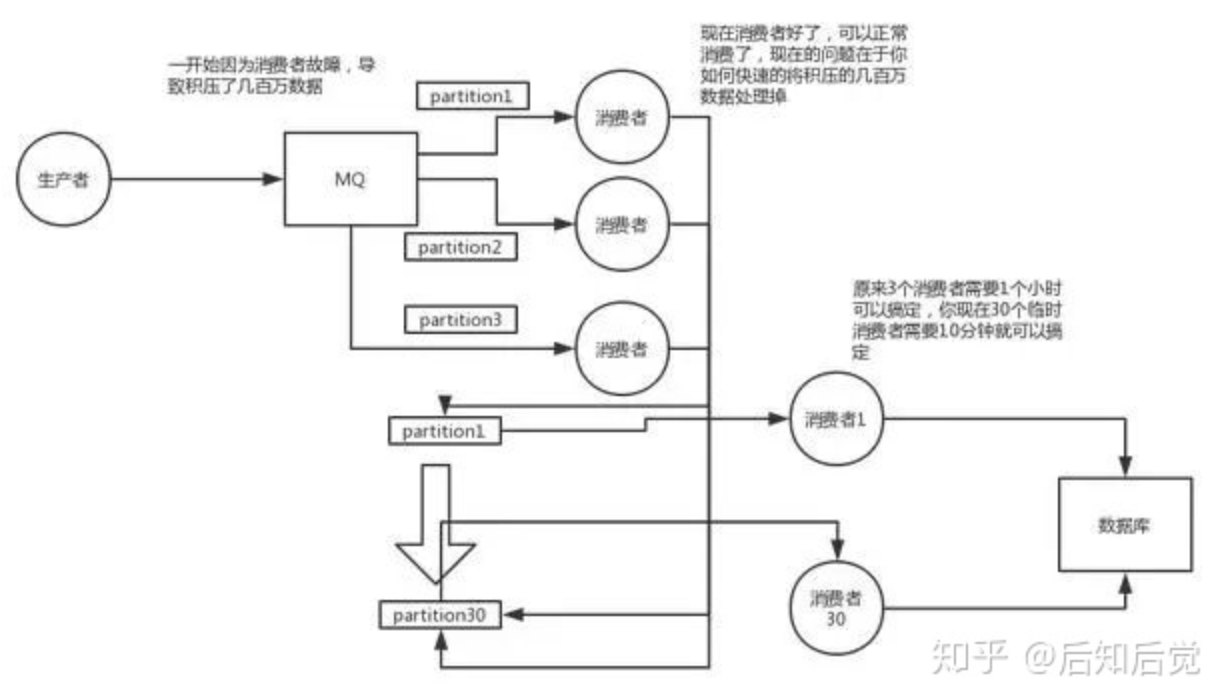
\includegraphics[width=1\textwidth]{fig/Message_Queue_1.png}
\end{figure}

\subsubsection{rabbitmq设置过期时间导致}
假设你用的是rabbitmq,rabbitmq是可以设置过期时间的,就是TTL,如果消息在queue中积压超过一定的时间就会被rabbitmq给清理掉,这个数据就没了。那这就是第二个坑了。这就不是说数据会大量积压在mq里,而是大量的数据会直接搞丢。

这个情况下,就不是说要增加consumer消费积压的消息,因为实际上没啥积压,而是丢了大量的消息。我们可以采取一个方案,就是批量重导,这个我们之前线上也有类似的场景干过。就是大量积压的时候,我们当时就直接丢弃数据了,然后等过了高峰期以后,比如大家一起喝咖啡熬夜到晚上12点以后,用户都睡觉了。

这个时候我们就开始写程序,将丢失的那批数据,写个临时程序,一点一点的查出来,然后重新灌入mq里面去,把白天丢的数据给他补回来。也只能是这样了。

假设1万个订单积压在mq里面,没有处理,其中1000个订单都丢了,你只能手动写程序把那1000个订单给查出来,手动发到mq里去再补一次。

\subsubsection{Queue快满了}
如果是消息积压在mq里,并且很长时间都没处理掉,此时导致mq都快写满了,咋办?这个还有别的办法吗?没有,谁让你第一个方案执行的太慢了,你临时写程序,接入数据来消费,消费一个丢弃一个,都不要了,快速消费掉所有的消息。然后走第二个方案,到了晚上再补数据吧。

\subsection{预防措施}
\begin{itemize}
\setlength{\itemsep}{0pt}
\setlength{\parsep}{0pt}
\setlength{\parskip}{0pt}
    \item 建延时队列,分担部分压力;
    \item 建立监控机制,队列消息堆积几百上千的时候就发出报警,及时的处理,不要让消息堆积过多
    \item ……
\end{itemize}


%\printbibliography
\bibliography{../ref}
\bibliographystyle{IEEEtran}
\end{document}